\documentclass{beamer}
\usepackage[utf8]{inputenc}

\usetheme{Madrid}
\usecolortheme{default}
\usepackage{amsmath,amssymb,amsfonts,amsthm}
\usepackage{txfonts}
\usepackage{tkz-euclide}
\usepackage{listings}
\usepackage{adjustbox}
\usepackage{array}
\usepackage{tabularx}
\usepackage{gvv}
\usepackage{lmodern}
\usepackage{circuitikz}
\usepackage{tikz}
\usepackage{graphicx}
\usepackage{caption}
\captionsetup{labelformat=empty}  % removes "Figure:"


\setbeamertemplate{page number in head/foot}[totalframenumber]

\usepackage{tcolorbox}
\tcbuselibrary{minted,breakable,xparse,skins}



\definecolor{bg}{gray}{0.95}
\DeclareTCBListing{mintedbox}{O{}m!O{}}{%
	breakable=true,
	listing engine=minted,
	listing only,
	minted language=#2,
	minted style=default,
	minted options={%
		linenos,
		gobble=0,
		breaklines=true,
		breakafter=,,
		fontsize=\small,
		numbersep=8pt,
		#1},
	boxsep=0pt,
	left skip=0pt,
	right skip=0pt,
	left=25pt,
	right=0pt,
	top=3pt,
	bottom=3pt,
	arc=5pt,
	leftrule=0pt,
	rightrule=0pt,
	bottomrule=2pt,
	toprule=2pt,
	colback=bg,
	colframe=orange!70,
	enhanced,
	overlay={%
		\begin{tcbclipinterior}
			\fill[orange!20!white] (frame.south west) rectangle ([xshift=20pt]frame.north west);
	\end{tcbclipinterior}},
	#3,
}
\lstset{
	language=C,
	basicstyle=\ttfamily\small,
	keywordstyle=\color{blue},
	stringstyle=\color{orange},
	commentstyle=\color{green!60!black},
	numbers=left,
	numberstyle=\tiny\color{gray},
	breaklines=true,
	showstringspaces=false,
}
\begin{document}

\title 
{4.7.42}
\date{October 1,2025}

\author 
{Navya Priya - EE25BTECH11045}
\graphicspath{./figs}

\frame{\titlepage}
\begin{frame}{Question}
   Find the length and the foot of perpendicular from the point $\brak{1,\frac{3}{2},2}$ to the plane $2\text{x}-2\text{y}+4\text{z}+5=0$. 
\end{frame}

\begin{frame}{Theoretical Solution}
Given plane equation $2\text{x}-2\text{y}+4\text{z}+5=0$ can be written as 
\begin{align}
    \vec{n}^\top\vec{x}=c
\end{align}
Where
\begin{align*}
    \vec{n}=\myvec{2\\-2\\4}\;\text{and}\;\text{c}=-5
\end{align*}
Let the point be $\vec{p}\myvec{1\\[3pt]\frac{3}{2}\\[3pt]2}$ and the point on the plane be $\vec{x}_o$. The equation of the line joining $\vec{p}$ and $\vec{x_o}$ is
\begin{align}
    \vec{x_o}\,=\,\vec{p}\,+\,\lambda\vec{n}
\end{align}
\end{frame}

\begin{frame}{Foot of Perpendicular}
    Multiply equation(2) on both sides by $\vec{n}^\top$
\begin{align}
\vec{n}^\top\brak{\vec{x_o}}\,=\,\vec{n}^\top\brak{\vec{p}\,+\,\lambda\vec{n}}
\end{align}
\begin{align}
\lambda\,=\,\frac{\vec{n}^\top\vec{x}_o}{\vec{n}^\top\vec{p}\,+\,\lambda\vec{n}^\top\vec{n}}
\end{align}
\begin{align}
     \lambda=\frac{-5}{\brak{2\,-2\,\,\,4}\myvec{1\\[3pt]\frac{3}{2}\\[3pt]2}\,+\,\lambda\brak{2\,-2\,\,\,4}\myvec{2\\-2\\4}}(\because \vec{n}^\top\vec{x_o}=-5)
\end{align}
\begin{align}
    \lambda\,=\,-\frac{1}{2}
\end{align}
\end{frame}

\begin{frame}{Foot of Perpendicular}
    Substitute the value of $\lambda$ in equation(2) to get $\vec{\text{x}}_o$
\begin{align}
    \vec{x}_o\,=\,\myvec{0\\[3pt]\frac{5}{2}\\[3pt]0}
\end{align}
\begin{align*}
    \therefore \textbf{Foot of perpendicular}\; \text{is}\; \vec{x}_o\,=\,\myvec{0\\[3pt]\frac{5}{2}\\[3pt]0}
    \end{align*}
\end{frame}

\begin{frame}{Length}
    The length of point $\myvec{1\\[3pt]\frac{3}{2}\\[3pt]2}$ to the plane $2\text{x}-2\text{y}+4\text{z}+5=0$ is
\begin{align}
    ||\vec{x_o}-\vec{p}||\,&=\,\sqrt{\brak{\vec{x_o}-\vec{p}}^\top\brak{\vec{x_o}-\vec{p}}}\\
    &=\sqrt{6}
\end{align}
\begin{align*}
    \therefore ||\vec{x_o}-\vec{p}||\,=\,\sqrt{6}
\end{align*}
\end{frame}

\begin{frame}[fragile]{C code}
\begin{lstlisting}
    #include <stdio.h>
#include <math.h>

void foot_and_length(double px, double py, double pz,
                     double a, double b, double c, double d,
                     double *x0, double *y0, double *z0, double *dist) {
    // Normal vector n = (a, b, c)
    double numerator = a*px + b*py + c*pz + d;
    double denominator = a*a + b*b + c*c;
    double lambda = - numerator / denominator;

    *x0 = px + lambda * a;
    *y0 = py + lambda * b;
    *z0 = pz + lambda * c;

    *dist = fabs(numerator) / sqrt(denominator);
}
\end{lstlisting}
\end{frame}

\begin{frame}[fragile]{C code}
\begin{lstlisting}
// For testing
int main() {
    double px = 1, py = 1.5, pz = 2;
    double a = 2, b = -2, c = 4, d = 5;
    double x0, y0, z0, dist;

    foot_and_length(px, py, pz, a, b, c, d, &x0, &y0, &z0, &dist);

    printf("Foot of perpendicular: (%.4f, %.4f, %.4f)\n", x0, y0, z0);
    printf("Perpendicular length: %.4f\n", dist);

    return 0;
}
\end{lstlisting}
\end{frame}

\begin{frame}[fragile]{CallC.py}
\begin{lstlisting}
    import ctypes

# Load the shared library
lib = ctypes.CDLL("./perpendicular.so")

# Define argument and return types
lib.foot_and_length.argtypes = [ctypes.c_double, ctypes.c_double, ctypes.c_double,
                                ctypes.c_double, ctypes.c_double, ctypes.c_double, ctypes.c_double,
                                ctypes.POINTER(ctypes.c_double),
                                ctypes.POINTER(ctypes.c_double),
                                ctypes.POINTER(ctypes.c_double),
                                ctypes.POINTER(ctypes.c_double)]

\end{lstlisting}
\end{frame}

\begin{frame}[fragile]{CallC.py}
\begin{lstlisting}

# Inputs
px, py, pz = 1.0, 1.5, 2.0
a, b, c, d = 2.0, -2.0, 4.0, 5.0

# Outputs
x0 = ctypes.c_double()
y0 = ctypes.c_double()
z0 = ctypes.c_double()
dist = ctypes.c_double()

# Call the C function
lib.foot_and_length(px, py, pz, a, b, c, d,
                    ctypes.byref(x0), ctypes.byref(y0), ctypes.byref(z0), ctypes.byref(dist))

print(f"Foot of perpendicular = ({x0.value:.4f}, {y0.value:.4f}, {z0.value:.4f})")
print(f"Length of perpendicular = {dist.value:.4f}")
\end{lstlisting}
\end{frame}

\begin{frame}[fragile]{Plot.py}
\begin{lstlisting}
    import numpy as np
import numpy.linalg as LA
import matplotlib.pyplot as plt
from mpl_toolkits.mplot3d import Axes3D

# Plane: 2x - 2y + 4z + 5 = 0
# Point: p(1, 3/2, 2)
p = np.array([1.0, 1.5, 2.0])
n = np.array([2.0, -2.0, 4.0])

# Foot of perpendicular (xo)
lam = - (np.dot(n, p) + 5) / np.dot(n, n)
xo = p + lam * n

# Distance (perpendicular length)
distance = abs(np.dot(n, p) + 5) / LA.norm(n)

# Create mesh for plane
x_vals = np.linspace(-2, 2, 40)
\end{lstlisting}
\end{frame}

\begin{frame}[fragile]{Plot.py}
\begin{lstlisting}
y_vals = np.linspace(0, 3.5, 40)
xx, yy = np.meshgrid(x_vals, y_vals)
zz = (-2*xx + 2*yy - 5)/4

# Plotting
fig = plt.figure(figsize=(9, 7))
ax = fig.add_subplot(111, projection='3d')

# Plane
ax.plot_surface(xx, yy, zz, alpha=0.5, color='lightblue')

# Scatter points
ax.scatter(*p, color='red', s=80, label='p(1, 3/2, 2)')
ax.scatter(*xo, color='blue', s=80, label=f'xo(0, 2.5, 0)')

# Perpendicular line pxo
ax.plot([p[0], xo[0]], [p[1], xo[1]], [p[2], xo[2]], 
        color='black', linestyle='--', linewidth=2, label='pxo ⟂ plane')
\end{lstlisting}
\end{frame}

\begin{frame}[fragile]{Plot.py}
\begin{lstlisting}
# ---- Draw right-angle square marker at xo ----
eps = 0.15  # size of the square
# Two perpendicular directions in the plane
u = np.cross(n, [1,0,0])
if LA.norm(u) == 0:
    u = np.cross(n, [0,1,0])
u = u / LA.norm(u)
v = np.cross(n, u)
v = v / LA.norm(v)

# Tiny square centered at xo
square_pts = [xo, xo + eps*u, xo + eps*u + eps*v, xo + eps*v, xo]
ax.plot([pt[0] for pt in square_pts], 
        [pt[1] for pt in square_pts], 
        [pt[2] for pt in square_pts], color="k")
\end{lstlisting}
\end{frame}

\begin{frame}[fragile]{Plot.py}
\begin{lstlisting}
# Annotations
ax.text(p[0]+0.05, p[1]+0.05, p[2]+0.05, "p(1, 3/2, 2)", color='red')
ax.text(xo[0]+0.05, xo[1]-0.15, xo[2]+0.05, "xo(0, 2.5, 0)", color='blue')

# Labels and title
ax.set_xlabel('X axis')
ax.set_ylabel('Y axis')
ax.set_zlabel('Z axis')
ax.set_title(f'Perpendicular from p to plane (Length = {distance:.4f})')
ax.legend()

plt.show()
\end{lstlisting}
\end{frame}

\begin{frame}{Plot}
From the graph, theoretical solution matches with the computational solution.

\begin{figure}[H]
\centering
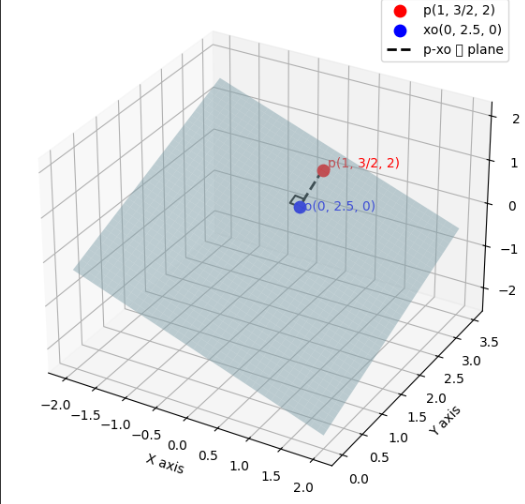
\includegraphics[width=0.5\columnwidth]{figs/graph.png}
\caption*{Perpendicular to the plane (length=$\sqrt{6}$)}
\label{fig:graph.png}
\end{figure} 
\end{frame}
\end{document}